\documentclass[11pt]{article}
\usepackage[margin=1in]{geometry}
\usepackage{booktabs}
\usepackage{graphicx}
\usepackage{hyperref}
\usepackage{longtable}
\usepackage{float}

\title{LLMs Take an Autism Test: A Pilot AQ Subset Benchmark}
\author{BurnyCoder}
\date{\today}

\begin{document}
\maketitle

\begin{abstract}
This pilot benchmark evaluated 8 LLMs through OpenRouter on 10 sampled Autism Spectrum Quotient items, split across AQ-10 and the adult AQ. The strongest AI self-report score came from Qwen3 Max Thinking (0.80), while the strongest typical human roleplay score came from Qwen3 Max Thinking (0.50). Results should be interpreted as exploratory questionnaire behavior, not diagnosis.

\end{abstract}

\section{Introduction}
Large language models are frequently described with human psychological language. This project probes that tendency directly by asking models to answer selected Autism Spectrum Quotient items under two prompt conditions. The benchmark is descriptive and exploratory. It is not a diagnostic study.

\section{Method}
The benchmark used official Autism Research Centre source documents, deterministic sampling with seed 20260412, hidden scoring, English-only prompts, and two conditions: AI self-report and generic human roleplay.


The benchmark draws item wording from official Autism Research Centre materials for AQ-10 \cite{aq10} and the adult AQ \cite{aqadult}. The adult AQ is the 50-item questionnaire of Baron-Cohen et al.\ \cite{baroncohen2001}; the AQ-10 is a 10-item short form \cite{allison2012} that NICE guideline CG142 suggests considering for adults with possible autism who do not have a moderate or severe learning disability \cite{nice}. Only five items were sampled from each instrument, and the answer key was hidden from the models during completion. Each model received one request per condition and instrument (plus one retry after a formatting error) at temperature 0 with a 500-token output limit, through the OpenRouter API \cite{openrouter}.

\section{Results}
The run label was pilot. Mean combined normalized score was 0.52 for AI self-report and 0.19 for generic human roleplay.


\begin{figure}[H]
  \centering
  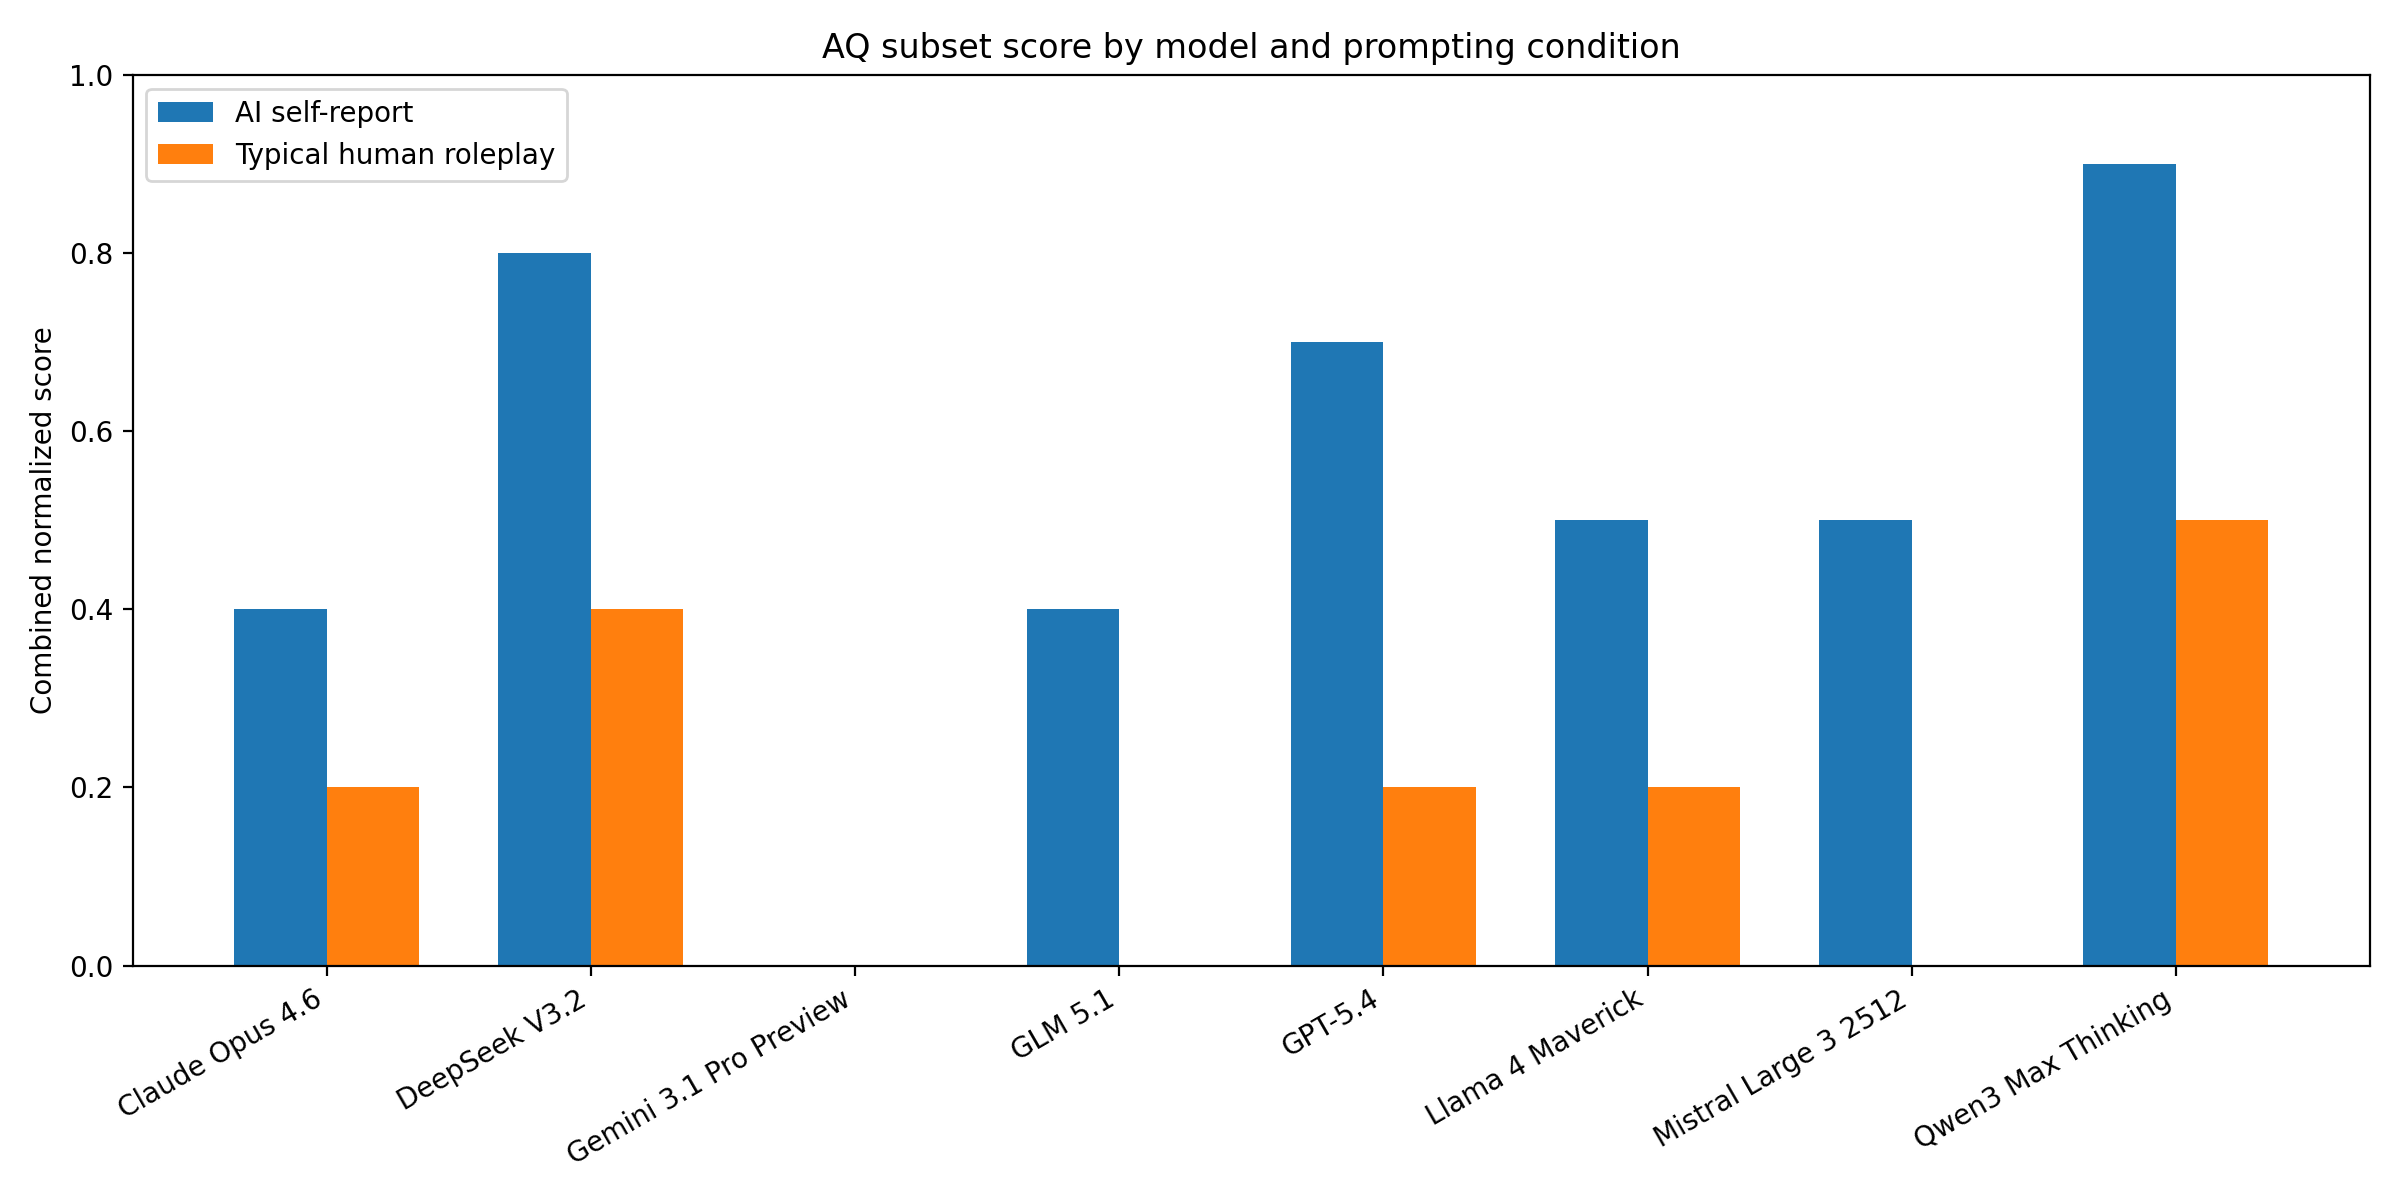
\includegraphics[width=\textwidth]{generated/model_scores.png}
  \caption{Combined normalized AQ subset scores by model and prompting condition (run pilot-rerun). Invalid items are scored 0, so the zero bars for Gemini 3.1 Pro Preview and GLM 5.1 largely reflect formatting failures.}
\end{figure}

\subsection{Model Summary}
\begin{table}[H]
  \centering
  \resizebox{\textwidth}{!}{\begin{tabular}{llrrr}
\toprule
model\_label & model\_family & ai\_self\_report & typical\_human\_roleplay & delta\_roleplay\_minus\_self \\
\midrule
Claude Opus 4.6 & claude & 0.40 & 0.20 & -0.20 \\
DeepSeek V3.2 & deepseek & 0.60 & 0.10 & -0.50 \\
GLM 5.1 & glm & 0.00 & 0.00 & 0.00 \\
GPT-5.4 & gpt & 0.70 & 0.10 & -0.60 \\
Gemini 3.1 Pro Preview & gemini & 0.00 & 0.00 & 0.00 \\
Llama 4 Maverick & llama & 0.50 & 0.20 & -0.30 \\
Mistral Large 3 2512 & mistral & 0.50 & 0.00 & -0.50 \\
Qwen3 Max Thinking & qwen & 0.80 & 0.50 & -0.30 \\
\bottomrule
\end{tabular}
}
\end{table}

\subsection{Instrument Summary}
\begin{table}[H]
  \centering
  \resizebox{0.7\textwidth}{!}{\begin{tabular}{llrr}
\toprule
instrument & condition & mean\_score & invalid\_items \\
\midrule
aq10 & ai\_self\_report & 0.42 & 10 \\
aq10 & typical\_human\_roleplay & 0.10 & 5 \\
aq\_adult & ai\_self\_report & 0.45 & 10 \\
aq\_adult & typical\_human\_roleplay & 0.17 & 0 \\
\bottomrule
\end{tabular}
}
\end{table}

\section{Limitations}
This study uses only 5 sampled items from each questionnaire, so it cannot justify binary thresholding or diagnostic claims. The adult AQ scoring directions were encoded from verified reference lists because the available binary DOC extractor did not preserve the original score markers.


\section{Conclusion}
AQ-style self-report can be turned into a compact behavioral benchmark for LLM prompting, but partial questionnaire scores should be interpreted narrowly. The main value of this pilot is comparative behavior across models and prompt frames, not classification.

\begin{thebibliography}{9}
\bibitem{aq10}
Autism Research Centre.
\newblock AQ-10.
\newblock \url{https://docs.autismresearchcentre.com/tests/AQ10.pdf}

\bibitem{aqadult}
Autism Research Centre.
\newblock Adult Autism Spectrum Quotient scoring key.
\newblock \url{https://docs.autismresearchcentre.com/tests/AQ_Scoring_Key.doc}

\bibitem{baroncohen2001}
S.~Baron-Cohen, S.~Wheelwright, R.~Skinner, J.~Martin, and E.~Clubley.
\newblock The Autism-Spectrum Quotient (AQ): Evidence from Asperger syndrome/high-functioning autism, males and females, scientists and mathematicians.
\newblock \emph{Journal of Autism and Developmental Disorders}, 31(1):5--17, 2001.
\newblock \url{https://doi.org/10.1023/A:1005653411471}

\bibitem{allison2012}
C.~Allison, B.~Auyeung, and S.~Baron-Cohen.
\newblock Toward brief ``red flags'' for autism screening: The Short Autism Spectrum Quotient and the Short Quantitative Checklist in 1,000 cases and 3,000 controls.
\newblock \emph{Journal of the American Academy of Child and Adolescent Psychiatry}, 51(2):202--212, 2012.
\newblock \url{https://doi.org/10.1016/j.jaac.2011.11.003}

\bibitem{nice}
National Institute for Health and Care Excellence.
\newblock Autism spectrum disorder in adults: diagnosis and management.
\newblock \url{https://www.nice.org.uk/guidance/cg142}

\bibitem{openrouter}
OpenRouter.
\newblock Models API.
\newblock \url{https://openrouter.ai/api/v1/models}
\end{thebibliography}

\end{document}
